\documentclass[11pt,french,english]{article}
\usepackage[T1]{fontenc}
\usepackage[utf8]{inputenc}
\usepackage{amssymb}
\usepackage{amsmath}
\usepackage{mathtools}
\usepackage{bbm}
\usepackage{ulem}
\usepackage{url}
\usepackage{graphicx}
\usepackage{enumerate}% http://ctan.org/pkg/enumerate
\usepackage{lmodern}
\usepackage[english]{babel}
\makeatletter
\addto\extrasfrench{%
   \providecommand{\og}{\leavevmode\flqq~}%
   \providecommand{\fg}{\ifdim\lastskip>\z@\unskip\fi~\frqq}%
}
\makeatother

\usepackage{etoolbox}
\newcommand{\points}[2]{\iftoggle{undergrad}{{\color{red}[#1 points]}}{{\color{red}[#2 points]}}}
\newcommand{\enfr}[2]{\iftoggle{french}{#2}{#1}}
\newcommand{\instruct}[1]{\iftoggle{final}{}{#1}}
\newcommand{\proftitle}[2]{\iftoggle{undergrad}{#1}{#2}}
% \newcommand{\question}[1]{\\ \textbf{Question.} #1}

\providecommand{\LyX}{L\kern-.1667em\lower.25em\hbox{Y}\kern-.125emX\@}

\makeatother

\usepackage{lmodern}
\usepackage[english]{babel}
\makeatletter
\addto\extrasfrench{%
   \providecommand{\og}{\leavevmode\flqq~}%
   \providecommand{\fg}{\ifdim\lastskip>\z@\unskip\fi~\frqq}%
}

\makeatother



\usepackage[colorinlistoftodos]{todonotes}

\usepackage{todonotes}
\newcommand{\ioannis}[1]{\todo[inline,color=green!40,caption={}]{{\it Ioannis:~}#1}}
\newcommand{\guillaume}[1]{\todo[inline,color=blue!40,caption={}]{{\it Guillaume:~}#1}}

\newcommand{\gradpoints}[1]{\textcolor{red}{Graduates #1 pts}}
\newcommand{\undergradpoints}[1]{\textcolor{orange}{Undergraduates #1 pts}}




% Switch this to false to hide answers
\iftrue
\newcommand{\answer}[1]{\\ \textbf{Answer.} #1 }
\else 
\newcommand{\answer}[1]{}
\fi

\usepackage[colorlinks=true]{hyperref}

\newcommand{\blue}[1]{{\color{blue}#1}}
\newcommand{\w}{\mathbf{w}}
\newcommand{\x}{\mathbf{x}}
\newcommand{\ith}[1]{^{(#1)}}

%%%%%%%%% STUDENTS CHANGE THIS

\providetoggle{undergrad}
\settoggle{undergrad}{false}     %%% "true" if 3395 or "false" if 6390

\providetoggle{french}
\settoggle{french}{false}        %%% "true" if french or "false" if english

\providetoggle{final}            
\settoggle{final}{false}        %%% "true" for your final homework submission (removes instructions)

%%%%%%%%%%%%%%%%%%%%% ^^^^^
\usepackage[colorlinks=true]{hyperref}

\DeclareMathOperator*{\argmax}{arg\,max}
\DeclareMathOperator*{\argmin}{arg\,min}

\begin{document}

\setlength{\parskip}{0.3cm} \setlength{\parindent}{0cm}

\begin{center}
\textbf{\proftitle{IFT 3395 Fondements de l'apprentissage machine \\ Prof. Guillaume Rabusseau}{IFT 6390 Fundamentals of Machine Learning \\ Ioannis Mitliagkas}}
\par\end{center}{\large \par}

\begin{center}
\textbf{\LARGE{\enfr{Homework 1 - Theoretical part}{Devoir 1 - Partie Th\'eorique}}}
\par\end{center}{\LARGE \par}



\paragraph{}

 

\instruct{
\paragraph{}
\begin{itemize}
\item \enfr{This homework must be done and submitted to Gradescope individually.
You are welcome to discuss with other students  \emph{but the solution you submit must be your own}.
Note that we will use Gradescope's plagiarism detection feature.
All suspected cases of plagiarism will be recorded and shared with university officials for further handling.\\}
{Ce devoir doit être fait et envoyé sur Gradescope individuellement. Vous pouvez discuter avec d'autres étudiants \emph{mais les réponses que vous soumettez doivent être les vôtres}. A noter que nous utiliserons l'outil de détection de plagiat de Gradescope. Tous les cas suspectés de plagiat seront enregistrés et transmis à l'Université pour vérification.}

\item \enfr{You need to submit your solution as a pdf file on Gradescope using the homework titled 
\iftoggle{undergrad}{\texttt{devoir theorique 1}}{\texttt{HW 1 - Theory}}.
\\}
{Vous devez soumettre vos solutions au format pdf sur Gradescope en utilisant le devoir intitulé \iftoggle{undergrad}{\texttt{devoir theorique 1}}{\texttt{HW 1 - Theory}}.}
\end{itemize}
}

\begin{enumerate}
\item \textbf{\enfr{Probability warm-up: conditional probabilities and Bayes rule}{Rappels de probabilités: probabilité conditionnelle et règle de Bayes}}
\points{5}{5}
\\

\begin{enumerate}
    \item \enfr{Give the definition of the conditional probability of a discrete random variable $X$ given a discrete random variable $Y$.}{Donnez la définition de la probabilité conditionnelle de la variable aléatoire discrète $X$ sachant la variable aléatoire discrète $Y$}
    \item \enfr{Consider a biased coin with probability $2/3$ of landing on heads and $1/3$ on tails. This coin is tossed three times. What is the probability that exactly two heads occur (out of the three tosses) given that the first outcome was a head?}{Soit une pièce déséquilibrée dont la probabilité d'obtenir face est $2/3$ et la probabilité d'obtenir pile est $1/3$. Cette pièce est lancée à trois reprises. Quelle est la probabilité d'obtenir exactement deux faces (parmi les trois lancers), sachant que le premier lancer a fait face ?}
    \item \enfr{Give two equivalent expressions of $P(X,Y)$:}{Donnez deux expressions équivalentes de $P(X,Y)$:}
    \begin{itemize}
        \item[(i)] \enfr{as a function of $\mathbb{P}(X)$ and $\mathbb{P}(Y |  X)$}{en fonction de $\mathbb{P}(X)$ et $\mathbb{P}(Y |  X)$}
        \item[(ii)] \enfr{as a function of $\mathbb{P}(Y)$ and $\mathbb{P}(X |  Y)$}{en fonction de $\mathbb{P}(Y)$ et $\mathbb{P}(X |  Y)$}
    \end{itemize}
    \item \enfr{Prove Bayes theorem:}{Prouvez le théorème de Bayes:}
    $$\mathbb{P}(X  |  Y) = \frac{\mathbb{P}(Y |  X)\mathbb{P}(X)}{\mathbb{P}(Y)}.$$
    
        \item \enfr{A survey of certain Montreal students is done, where 55\% of the surveyed students are affiliated with UdeM while the others are affiliated with McGill. A student is drawn randomly from this surveyed group.}
        {Un sondage des étudiants Montréalais est fait, où 55\% des élèves sondés sont affiliés à l'UdeM alors que les autres sont affiliés à McGill. Un étudiant est choisi aléatoirement parmis ce groupe.}
        \begin{enumerate}
            \item \enfr{What is the probability that the student is affiliated with McGill?}{Quelle est la probabilité que l'étudiant soit affilié à McGill?}
            \item  \enfr{Now let's say that this student is bilingual, and you know that 80\% of UdeM students are bilingual while 50\% of McGill students are. Given this information, what is the probability that this student is affiliated with McGill ?}{Considérons maintenant que l'étudiant est bilingue, et que 80\% des étudiants de l'UdeM sont bilingues alors que seulement 50\% des étudiants de McGill le sont. Étant donné cette information, quelle est la probabilité que cet étudiant soit affilé à McGill ?}
        \end{enumerate}
        
\end{enumerate}


\begin{enumerate}[(a)]
    \item $$P(X=x | Y=y) = \frac{P(X=x) \cap P(Y=y)}{P(Y=y)}$$
    \item Let $T_n$ be the result of the nth toss.
    \begin{align*}
        P((T_1 = H, T_2 = T) or (T_1 = T, T_2 = H)| T_0 = H) &= \frac{P(HHT) + P(HTH)}{P(H)} \\
        &= \frac{2*(1/3)^1*(2/3)^2}{(2/3)} \\
        &= \fbox{4/9}
    \end{align*}
    \item (i) $$P(X,Y) = P(Y,X) = P(Y|X)P(X)$$ (ii) $$P(X,Y) = P(X|Y)P(Y)$$
    \item $$P(X|Y) = \frac{P(X \cap Y)}{P(Y)} = \frac{P(Y \cap X)}{P(Y)} = \frac{P(Y|X)P(X)}{P(Y)} \qquad \square$$ 
    \item (i) $$P(McGill) = 1 - P(UdeM) = \fbox{0.45}$$ (ii) 
    \begin{align*}
        P(McGill | bilingual) &= \frac{McGill \cap bilingual}{P(bilingual)} \\
        &= \frac{P(McGill \cap bilingual)P(Mcgill)}{P(bilingual)} \\
        &= \frac{P(McGill \cap bilingual)P(Mcgill)}{P(McGill \cap bilingual)P(Mcgill) + P(UdeM \cap bilingual)P(UdeM)} \\
        &= \frac{(0.50)(0.45)}{(0.50)(0.45) + (0.80)(0.55)} \\
        &= \fbox{45/133}
    \end{align*}
\end{enumerate}

\item \textbf{\enfr{Bag of words and single topic model}{Bag of words (sac de mots) et modèle de sujet unique}} %
\points{20}{12}
\\

\enfr{We consider a classification problem where we want to predict the topic of a document from a given corpus (collection of documents).
The topic of each document can either be \textit{sports} or \textit{politics}. 2/3 of the documents in the corpus are about \textit{sports} and 1/3 are about \textit{politics}.

We will use a very simple model where we ignore the order of the words appearing in a document and we assume that words in a document are independent from one another given the topic of the document.

In addition, we will use very simple statistics of each document as features: the probabilities that a word chosen randomly in the document is either "goal", "kick", "congress", "vote", or any another word~(denoted by \textit{other}).
We will call these five categories the \emph{vocabulary} or \emph{dictionary} for the documents: $V=\{"goal","kick ", "congress", "vote", \textit{other}\}$.

Consider the following distributions over words in the vocabulary given a particular topic:
}{On s'intéresse à un problème de classification où l'on veut prédire le sujet d'un document d'un certain corpus (ensemble de documents).
Le sujet de chaque document peut être soit \textit{sport}, soit \textit{politique}. 2/3 des documents du corpus sont sur le \textit{sport}, et 1/3 sont sur la \textit{politique}. 

On va utiliser un modèle très simple où on ignore l'ordre des mots apparaissant dans le document et l'on considère que les mots dans un document sont indépendants les uns des autres, étant donné le sujet du document.

De plus, nous allons utiliser des statistiques très simples des documents: les probabilités qu'un mot choisi au hasard dans un document soit "goal", "kick", "congress", "vote", ou n'importe quel autre mot (dénoté par \textit{other}). Nous appelons ces cinq catégories le \emph{vocabulaire} ou \emph{dictionnaire} pour les documents: $V=\{"goal","kick ", "congress", "vote", \textit{other}\}$.

Soit les distributions suivantes des mots du vocabulaire, par sujet:}


\begin{center}
\begin{table}[h!]
\begin{tabular}{l|cc}
     & $\mathbb{P}(\mathrm{word} \mid \mathrm{topic}=\textit{sports})$ & $\mathbb{P}(\mathrm{word} \mid \mathrm{topic}=\textit{politics})$\\
     \hline 
$\mathrm{word} = "goal"$    & $3/200$& $8/1000$ \\
$\mathrm{word} = "kick"$    & $1/200$& $2/1000$ \\
$\mathrm{word} = "congress"$    & $0$& $1/50$ \\
$\mathrm{word} = "vote"$    & $5/1000$& $2/100$ \\
$\mathrm{word} = \textit{other}$  & $960/1000$ & $950/1000$ 
\end{tabular}
    \caption{}
    \label{tab:bow}
\end{table}
\end{center}

\enfr{This table tells us for example that the probability that a word chosen at random in a document is "vote" is only 5/1000 if the topic of the document is \textit{sport}, but it is 2/100 if the topic is \textit{politics}.}{Cette table nous dit par exemple que la probabilité qu'un mot choisi aléatoirement dans un document soit "vote" n'est que de 5/1000 si le sujet du document est le \textit{sport}, mais est de 2/100 si le sujet est la \textit{politique}.}

\begin{enumerate}
 
\item \enfr{What is the probability that a random word in a document is "goal" given that the topic is \textit{politics}?} {Quelle est la probabilité qu'un mot aléatoire dans un document soit "goal" étant donné que le sujet est la \textit{politique} ?}

\item \enfr{In expectation, how many times will the word "goal" appear in a document containing 200 words whose topic is \textit{sports}?}{Quelle est l'espérance du nombre de fois où le mot "goal" apparait dans un document de 200 mots dont le sujet est le \textit{sport}?}

\medskip
\item \enfr{We draw randomly a document from the corpus. What is the probability that a random word of this document is "goal"?} {On tire aléatoirement un document du corpus. Quelle est la probabilité qu'un mot aléatoire de ce document soit "goal"?}

\item \enfr{Suppose that we draw a random word from  a document and this word is "kick". What is the probability that the topic of the document is \textit{sports}?} {Supposons que l'on tire aléatoirement un mot d'un document et que ce mot est "kick". Quelle est la probabilité que le sujet du document soit le \textit{sport}?}

\item \enfr{Suppose that we randomly draw two words from a document and the first one is "kick". What is the probability that the second word is "goal"? }{Supposons que l'on tire aléatoirement deux mots d'un document et que le premier soit "kick". Quelle est la probabilité que le second mot soit "goal"?}

\item \enfr{Going back to learning, suppose that you do not know the conditional probabilities given a topic or the probability of each topic (i.e. you don't have access to the information in table 1 or the topic distribution), but you have a dataset of $N$ documents where each document is labeled with one of the topics \textit{sports} and \textit{politics}.
How would you estimate the conditional probabilities~(e.g., $\mathbb{P}(\mathrm{word} = "goal" \mid \mathrm{topic}=\textit{politics})$) and topic probabilities~(e.g., $\mathbb{P}(\mathrm{topic}=\textit{politics})$) from this dataset?} {Pour en revenir à l'apprentissage, supposons que l'on ne connaisse pas les probabilités conditionnelles étant donné chaque sujet ni les probabilités de chaque sujet (i.e. nous n'avons pas accès aux informations de la table 1 où aux proportions de chaque sujet), mais nous avons un jeu de données de $N$ documents où chaque document est annoté avec un des sujet \textit{sport} ou \textit{politique}.
Comment estimeriez vous les probabilités conditionnelles~(e.g., $\mathbb{P}(\mathrm{mot} = "goal" \mid \mathrm{sujet}=\textit{politique})$) et les probabilités des sujets~(e.g., $\mathbb{P}(\mathrm{sujet}=\textit{politique})$) à partir de ce jeu de données ?} \\

\end{enumerate}

\begin{enumerate}[(a)]
    \item $$P("goal" | politics) = \frac{8}{1000}$$
    \item $$200*P("goal" | sports) = 200\left(\frac{3}{200}\right) = 3$$
    \item \begin{align*}
        P("goal") &= P("goal"|sports)P(sports) + P("goal"|politics)P(politics) \\
        &= \left(\frac{3}{200}\right)\left(\frac{2}{3}\right) + \left(\frac{8}{1000}\right)\left(\frac{1}{3}\right) \\
        &= 0.0127
    \end{align*}
    \item \begin{align*}
        P(sports|"kick") &= \frac{P("kick"|sports)P(sports)}{P("kick"|sports)P(sports) + P("kick"|politics)P(politics)}\\
        &= \frac{\frac{1}{200}*\frac{2}{3}}{\frac{1}{200}*\frac{2}{3} + \frac{2}{1000}*\frac{1}{3}} \\
        &= \frac{5}{6}
    \end{align*}
    \item Since words are independent, we can ignore the fact that the first word chosen was "kick" and it will suffice to calculate P("goal"). As in $2(c)$, $$P("goal") = 0.0127$$
    \item For the conditional probabilities, we would take a count of all words in each of the 2 document classes then divide that by the total number of words found in all documents per document class. i.e. $$P("goal"|politics) = \frac{\text{\# instances of "goal" in all politics documents}}{\text{\# words in all politics documents}}$$\par
    For the topic probabilities, it would suffice to get a count of the number of documents classified as politics and sports and take the quotient of those totals and N. i.e. $$P("politics") = \frac{\text{\# labels = politics}}{N}$$
\end{enumerate}

\item \textbf{\enfr{Maximum likelihood estimation}{Estimateur du maximum de vraisemblance}}
\points{10}{5}
\\

\enfr{Let $\x\in \mathbb{R}^2$ be uniformly distributed over a diamond area with diagonals $2\theta$ where $\theta$ is a parameter as shown in the figure. That is, the pdf of $\x$ is given by
$$
f_\theta(\x) = \begin{cases}
1/2\theta^2&\text{if } ||\x||_1 \leq \theta\\
0&\text{otherwise}
\end{cases}
$$
where $||\x||_1 = |x_1| + |x_2|$ is the L1 norm.
}
{Soit $x\in \mathbb{R}^2$ distribué uniformément dans l'aire du diamant avec les diagonales $2\theta$, $\theta$ un paramètre, tel que montré dans la figure. C'est-à-dire, la distribution de $\x$ est donnée par
$$
f_\theta(\x) = \begin{cases}
1/2\theta^2&\text{si } ||\x||_1 \leq \theta\\
0&\text{sinon}
\end{cases}
$$
où $||\x||_1 = |x_1| + |x_2|$ est la norme $\ell_1$ de $\mathbf{x}$.
}

\begin{figure}[ht]
\centering
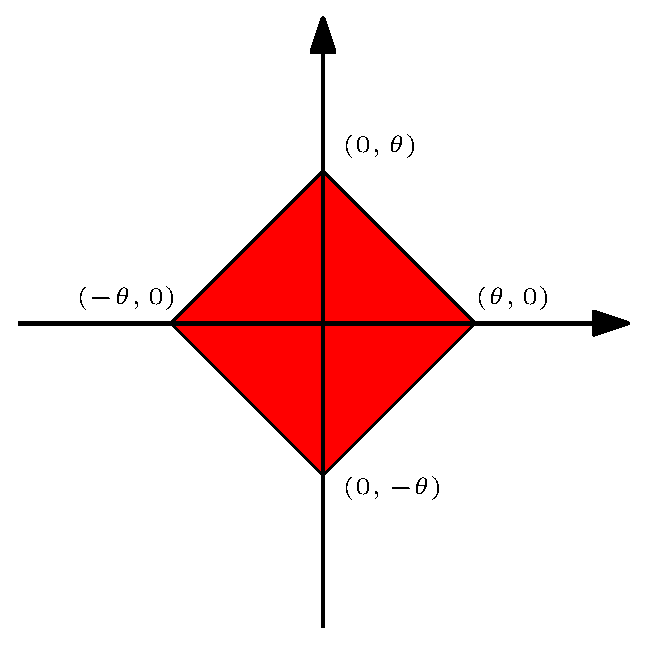
\includegraphics[width = 0.5\textwidth]{diamond.eps}
\end{figure}

\enfr{Suppose that $n$ samples $D=\{ \x_1, \dots, \x_n\}$ are drawn \emph{independently} according to $f_\theta(\x)$.}
{Supposons que $n$ points $D=\{ \x_1, \dots, \x_n\}$ sont tirés aléatoirement \emph{indépendemment} selon $f_\theta(\x)$.}

\begin{enumerate}

\item \enfr{Let $f_\theta(\x_1, \x_2, \ldots, \x_n)$ denote the joint pdf of $n$ independent and identically distributed (i.i.d.)\ samples drawn according to $f_\theta(\x)$.
Express $f_\theta(\x_1, \x_2, \ldots, \x_n)$ as a function of $f_\theta(\x_1), f_\theta(\x_2), \ldots, f_\theta(\x_n)$}
{Soit $f_\theta(\x_1, \x_2, \ldots, \x_n)$ la fonction de densité de probabilité jointe de $n$ points indépendemment et identiquement distribué (i.i.d) selon $f_\theta(\x)$.
Exprimez $f_\theta(\x_1, \x_2, \ldots, \x_n)$ en fonction de $f_\theta(\x_1), f_\theta(\x_2), \ldots, f_\theta(\x_{n-1})$}

\item \enfr{We define the \emph{maximum likelihood estimate} by the value of $\theta$ which maximizes the likelihood of having generated the dataset $D$ from the distribution $f_\theta(\x)$. Formally,
$$\theta_{MLE} = \argmax_{\theta \in \mathbb{R}^+} f_\theta(\x_1,\x_2,\ldots,\x_n),$$
Find the maximum likelihood estimate of $\theta$.}%
{On définie \emph{l'estimateur du maximum de vraisemblance} comme la valeur de $\theta$ qui maximise la vraisemblance de générer le jeu de donnée $D$ à partir de la distribution $f_\theta(\x)$. Formellement,
$$\theta_{MLE} = \argmax_{\theta \in \mathbb{R}} f_\theta(\x_1,\x_2,\ldots,\x_n),$$
Trouvez l'estimateur du maximum de vraisemblance de $\theta$.}
\end{enumerate}

\begin{enumerate}[(a)]
    \item \begin{align*}
        L(\theta) &= f_{\theta}(x_1, x_2, \ldots, x_n) \\
        &= \prod_{i=1}^{n} f_{\theta}(x_i) \\
        &= \left(\frac{1}{2\theta^2}\right)\left(\frac{1}{2\theta^2}\right) \ldots \left(\frac{1}{2\theta^2}\right)
    \end{align*}
    \[L(\theta) = 
        \begin{cases} 
            \frac{1}{(2\theta^2)^n} & ||x_i||_1 \leq \theta \quad i = (1, \ldots, n)\\
            0 & \text{Otherwise}
        \end{cases}
    \]
    \item We can see that the value of $\theta$ that will maximize $L(\theta)$ will have to be the smallest value of $\theta$ such that $\theta \geq ||x_i||_1$. Therefore, 
    $$\hat\theta = max(||x_1||_1, ||x_2||_1, \ldots, ||x_n||_1)$$
\end{enumerate}


\item \textbf{\enfr{Maximum likelihood meets histograms}{Estimateur du maximum de vraisemblance et histograme}}
\points{10}{10}
\\

\enfr{Let $X_1, X_2, \cdots, X_n$  be $n$ i.i.d data points drawn from a piece-wise constant probability density function over $N$ equal size bins between 0 and 1 ($B_1, B_2, \cdots, B_N$), where the constants are $\theta_1, \theta_2, \cdots, \theta_N$.}
{Soit le jeu de données $X_1, X_2, \cdots, X_n$ sont $n$ données i.i.d tirées d'une distribution de probabilité constante par morceaux. Il y a $N$ morceaux de longueur égale entre 0 et 1 ($B_1, B_2, \cdots, B_N$), où les constantes sont $\theta_1, \theta_2, \cdots, \theta_N$.}
$$
p(x;\theta_1, \cdots, \theta_N) = 
\begin{cases} 
\theta_j 	&\frac{j-1}{N} \leq x  < \frac{j}{N} \mbox{ for } j \in \{1, 2, \cdots, N\}\\
0 		&\mbox{otherwise} 
\end{cases}
$$
\enfr{We define $\mu_j$ for $j \in \{1, 2, \cdots, N\}$ as $\mu_j \coloneqq  \sum_{i=1}^n \mathbbm{1}(X_i \in B_j).$}
{On défini $\mu_j$ pour $j \in \{1, 2, \cdots, N\}$ en tant que $\mu_j \coloneqq  \sum_{i=1}^n \mathbbm{1}(X_i \in B_j).$}

\begin{enumerate}
\item \enfr{Using  the fact that the total area underneath a probability density function is 1, express $\theta_N$ in terms of the other constants.}
{Utilisant le fait que l'aire totale sous une distribution de probabilité est 1, exprimez $\theta_N$ en fonction de $\theta_1, \theta_2, \cdots,  \theta_{N-1}$.}
\item \enfr{Write down the log-likelihood of the data in  terms of $\theta_1, \theta_2, \cdots,  \theta_{N-1}$ and $\mu_1, \mu_2, \cdots,  \mu_{N-1}$.}
{Écrivez le log-vraisemblance du jeu de données en fonction de $\theta_1, \theta_2, \cdots,  \theta_{N-1}$ et $\mu_1, \mu_2, \cdots,  \mu_{N-1}$.}
\item \enfr{Find the maximum likelihood estimate of $\theta_j$ for $j \in \{1, 2, \cdots, N\}.$ }
{Trouvez l'estimateur du maximum de vraisemblance de $\theta_j$, $j \in \{1, 2, \cdots, N\}.$}
\end{enumerate}

\item \textbf{\enfr{Histogram methods}{Méthodes à base d'histogrames}} %
\points{10}{10}
\\

\enfr{Consider a dataset $\{x_j\}_{j=1}^n$ where each point $x \in [0, 1]^d$. Let $f(x)$ be the true unknown data distribution. You decide to use a histogram method to estimate the density $f(x)$ and divide each dimension into $m$ bins.}
{Soit le jeu de données $\{x_j\}_{j=1}^n$ où chaque point $x \in [0, 1]^d$. La fonction $f(x)$ représente la vraie distribution inconnue des données. Vous décidez d'utiliser une méthode à base d'histogramme pour estimer $f(x)$. Chaque dimension est divisée en $m$ régions.}

\begin{enumerate}
    \item \enfr{Show that for a measurable set $S$, $\mathbb{E}_{x\sim f}[\mathbbm{1}_{\{x \in S\}}] = \mathbb{P}_{x\sim f}(x \in S)$, where $\mathbbm{1}_{\{x \in S\}}=1$ if $x\in S$ and $0$ otherwise.}{Démontrez que pour un ensemble mesurable $S$, $\mathbb{E}_{x\sim f}[\mathbbm{1}_{\{x \in S\}}] = \mathbb{P}_{x\sim f}(x \in S)$, où $\mathbbm{1}_{\{x \in S\}}=1$ si $x\in S$ et $0$ sinon.}
    \item \enfr{Combining the result of the previous question with the Law of Large Numbers, show that the estimated probability of falling in bin $i$, as given by the histogram method, tends to $\mathbb{P}_{x\sim f}(x \in V_i)=\int_{V_i} f(x)dx$, the true probability of falling in bin $i$, as $n \rightarrow \infty$. $V_i$ denotes the volume occupied by bin $i$.}{En combinant le résultat de la question précédente avec la loi des grands nombres, démontrez que la probabilité estimée d'être dans la région $i$, telle que donnée par les méthodes à base d'histogramme, tend vers $\mathbb{P}_{x\sim f}(x \in V_i)=\int_{V_i} f(x)dx$, la vraie probabilité d'être dans la région $i$, lorsque $n \rightarrow \infty$. $V_i$ est le volume occupé par la région $i$.}
    \item \enfr{Consider the MNIST dataset with 784 dimensions~(i.e. $x\in [0,1]^{784}$). We divide each dimension into 2 bins. How many digits (base 10) does the total number of bins have?}{Soit le jeu de données MNIST, où chaque point vit en 784 dimensions~(i.e. $x\in [0,1]^{784}$). Nous divisons chaque dimensions en 2 régions. Combien de chiffres (en base 10) contient le nombre total de régions?}
    \item \enfr{Assuming a uniform distribution over all bins, how many data points would you need to get $k$ points per bin on average?}{Assumant une distribution uniforme sur toutes les régions, combien de données faut il pour avoir $k$ données par région en moyenne?}
    \item \enfr{Assuming a uniform distribution over all bins, what is the probability that a particular bin is empty, as a function of $d$, $m$ and $n$?}{Assumant une distribution uniforme sur tous les régions, quelle est la probabilité qu'une région donnée soit vide, en fonction de $d$, $m$ et $n$?}
\end{enumerate}

\item \textbf{\enfr{Gaussian Mixture}{Mélange de Gaussiennes}} %
\points{0}{10}
\\

\enfr{Let $\mu_{0}, \mu_{1} \in \mathbb{R}^{d}$, and let $\Sigma_{0}, \Sigma_{1}$ be two $d \times d$ positive definite matrices (i.e. symmetric with positive eigenvalues). \\
We now introduce the two following pdf over $\mathbb{R}^{d}$ :}
{Soit $\mu_{0}, \mu_{1} \in \mathbb{R}^{d}$, et soit $\Sigma_{0}, \Sigma_{1}$ deux matrices $d \times d$ positives définies (i.e. symmétriques avec des valeurs propres strictement positives). \\
On définie maintenant les deux fonctions de densités de probabilités suivantes sur $\mathbb{R}^{2}$:} \\

$$f_{\mu_{0},\Sigma_{0}}(\x)=\frac{1}{(2\pi)^{\frac{d}{2}}\sqrt{det(\Sigma_{0})}}e^{-\frac{1}{2}(\x-\mu_{0})^{T}\Sigma_{0}^{-1}(\x-\mu_{0})}$$ \\
$$f_{\mu_{1},\Sigma_{1}}(\x)=\frac{1}{(2\pi)^{\frac{d}{2}}\sqrt{det(\Sigma_{1})}}e^{-\frac{1}{2}(\x-\mu_{1})^{T}\Sigma_{1}^{-1}(\x-\mu_{1})}$$

\enfr{These pdf correspond to the multivariate Gaussian distribution of mean $\mu_{0}$ and covariance $\Sigma_{0}$, denoted $\mathcal{N}_{d}(\mu_{0},\Sigma_{0})$, and the multivariate Gaussian distribution of mean $\mu_{1}$ and covariance $\Sigma_{1}$, denoted $\mathcal{N}_{d}(\mu_{1},\Sigma_{1})$.}
{Ces fonctions de densité de probabilités correspondent à la distribution gaussienne multivariée de centre $\mu_0$ et covariance $\Sigma_0$, notée $\mathcal{N}_{d}(\mu_{0},\Sigma_{0})$, et à la gaussienne multivariée de centre $\mu_{1}$ et covariance $\Sigma_{1}$, notée $\mathcal{N}_{d}(\mu_{1},\Sigma_{1})$.}

\enfr{We now toss a balanced coin $Y$, and draw a random variable $X$ in $\mathbb{R}^{d}$, following this process : if the coin lands on tails ($Y=0$) we draw $X$ from $\mathcal{N}_{d}(\mu_{0},\Sigma_{0})$, and if the coin lands on heads ($Y=1$) we draw $X$ from $\mathcal{N}_{d}(\mu_{1},\Sigma_{1})$.}
{On lance maintenant une pièce équilibrée $Y$, et on tire une variable aléatoire $X$ dans $\mathbb{R}^{d}$, en suivant le procédé suivant : si la pièce atterit sur pile ($Y=0$), on tire $X$ selon $\mathcal{N}_{d}(\mu_{0},\Sigma_{0})$, et si la pièce atterit sur face ($Y=1$), on tire $X$ selon $\mathcal{N}_{d}(\mu_{1},\Sigma_{1})$. }

\begin{enumerate}
\item \enfr{Calculate $\mathbb{P}(Y=0|X=\x)$, the probability that the coin landed on tails given $X=\x\in\mathbb{R}^{d}$, as a function of $\mu_{0}$, $\mu_{1}$, $\Sigma_{0}$, $\Sigma_{1}$, and $\x$. 
Show all the steps of the derivation.}
{Calculez $\mathbb{P}(Y=0|X=\x)$, la probabilité que la pièce atterisse sur pile sachant $X=\x\in\mathbb{R}^{2}$, en fonction de $\mu_{0}$, $\mu_{1}$, $\Sigma_{0}$, $\Sigma_{1}$, et $\x$.
Montrez toutes les étapes du calcul.}

\item \enfr{Recall that the Bayes optimal classifier is $h_{Bayes}(\x) = \underset{y \in \{0,1\}}{\mathrm{argmax}}\ \mathbb{P}(Y=y|X=\x)$. Show that in this setting if $\Sigma_0 = \Sigma_1$ the Bayes optimal classifier is linear in $\x$.}%
{Rappelez-vous que le classifieur optimale Bayes est $h_{Bayes}(\x) = \underset{y \in \{0,1\}}{\mathrm{argmax}}\ \mathbb{P}(Y=y|X=\x)$. Assumant $\Sigma_0 = \Sigma_1$, Démontrez que le classifieur optimal Bayes est linéaire en $\x$. }
\end{enumerate}
\end{enumerate}

%%%%%%%%%%%%%%%%%%%%%%%%%%%%%%%%%%%%%%%%%%%%%%%%%%%%%%%%%%%%%




\end{document}